\chapter{Results}
\section{Evaluation of Performance of The Augmented CNN Models}
In this section we will evaluate the augmented CNN models and compare and contrast with the original models.  The section is broken into subsections for each datasets CNN models.
\subsection{Radiography CNN Models}
  The non-augmented radiography dataset was imbalanced so a total of 6,570 images were generated for the COVID X-rays and masks and a total of 8,840 pneumonia X-ray and mask images were generated to bring both classes in relative balance with the Normal class.  The augmented dataset will be off by a around 5-10 images for augmented classes due to computational issues when trying to generate all files at once but the results still show a big improvement in some models.  The augmented dataset contains 60,933, while the original dataset contained only 30,306. 
\subsubsection{Radiography Baseline Model}
The radiography baseline model ran for 10 epochs with 1333 steps per epoch and attained a final training set accuracy of 0.9314 and a final training set loss of 0.1663 along with a final validation set accuracy of 0.9200 and a validation set loss of 0.2200.  The  model achieved a test set accuracy of 0.9222 and a test set loss of 0.2068 when the dataset was augmented.  In comparison to the original model which has a training set accuracy of 0.8611 and a training loss of 0.3446 and a validation set accuracy of  0.8306 and a validation set loss of 0.4120 and a test set accuracy of 0.8434 and a test set loss of 0.3801  when trained for the same amount of epochs on the non-augmented set. The model trained on the augmented set shows a clear improvement in terms of accuracy and of loss.  The training accuracy increased by 0.0703 and the training loss decreased by 0.1683 along with the validation accuracy increasing by 0.0894 and the loss decreased by 0.192. The test set accuracy also increased by 0.0788 and the test set loss was lowered by 0.1732 when training on the augmented dataset.  In this case the augmented model shows a clear improvement over the original baseline model. The training and validation accuracy along with the training and validation loss of this model are shown below.
 \begin{figure}[H]
    \centering    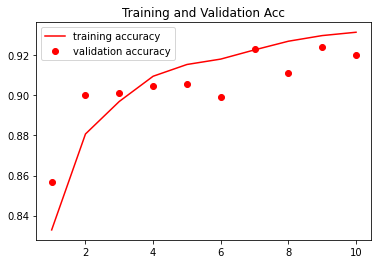
\includegraphics[width=1\textwidth,height=5cm,keepaspectratio]{Images/RadiographyCNNBaselineTrainAndValAccAugmentedDCGAN.png}\\
    \caption{Radiography Augmented Baseline Model DCGAN Accuracy - The X-Axis shows the epoch number and the Y-axis shows the accuracy}
    \label{fig:Radiography Augmented Baseline Model DCGAN Accuracy}
\end{figure}
 \begin{figure}[H]
    \centering
    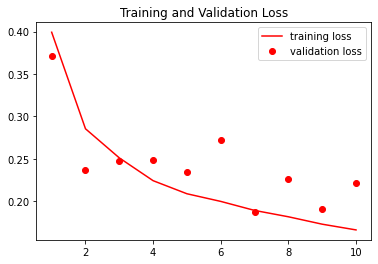
\includegraphics[width=1\textwidth,height=5cm,keepaspectratio]{Images/RadiographyCNNBaselineTrainAndValLossAugmentedDCGAN.png}\\
    \caption{Radiography Augmented Baseline Model DCGAN Loss - The X-Axis shows the epoch number and the Y-axis shows the loss}
    \label{fig:Radiography Augmented Baseline Model DCGAN Loss}
\end{figure}
\subsubsection{Radiography Xception Model}
The augmented Radiography Xception model attained a final training set accuracy of 0.9699 and a final training set loss of 0.0776 alongside a final validation accuracy of 0.9435 and a final validation loss of 0.1365 after 10 epochs.  The model also achieved a final test set accuracy of 0.9464 and a test set loss of 0.1369.  In comparison the original model attained a training set accuracy of 0.9543 and a training set loss of 0.1162  alongside a validation set accuracy of 0.8964 and a validation set loss of 0.3867.  The original model also had a test set accuracy of 0.9002 and a test set loss of 0.3833.  The augmented model shows an increase of 0.0156 for the training accuracy and a decrease of 0.0386 for the training loss.  The validation set accuracy had an increase of 0.0471 and the validation set loss had an decrease of 0.2502. The model also performed better on the test set with accuracy increasing by 0.0462 and loss decreasing by 0.2464.  Again this model outperformed the original non-augmented model. Figure \ref{fig:Radiography Augmented Xception Model DCGAN Accuracy} shows the training and validation accuracy and figure \ref{fig:Radiography Augmented Xception Model DCGAN Loss} shows the training and validation loss.
 \begin{figure}[H]
    \centering    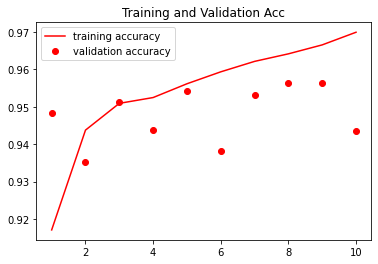
\includegraphics[width=1\textwidth,height=5cm,keepaspectratio]{Images/RadiographyCNNXceptionTrainAndValAccAugmentedDCGAN.png}\\
    \caption{Radiography Augmented Xception Model DCGAN Accuracy - The X-Axis shows the epoch number and the Y-axis shows the accuracy}
    \label{fig:Radiography Augmented Xception Model DCGAN Accuracy}
\end{figure}
 \begin{figure}[H]
    \centering
    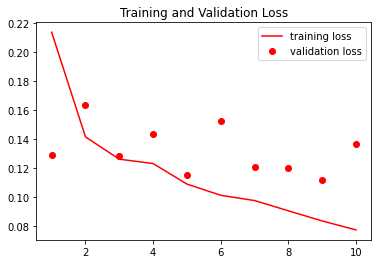
\includegraphics[width=1\textwidth,height=5cm,keepaspectratio]{Images/RadiographyCNNXceptionTrainAndValLossAugmentedDCGAN.png}\\
    \caption{Radiography Augmented Xception Model DCGAN Loss - The X-Axis shows the epoch number and the Y-axis shows the loss}
    \label{fig:Radiography Augmented Xception Model DCGAN Loss}
\end{figure}
\subsubsection{Radiography ResNet50V2 Model}
The augmented radiography ResNet50V2 Model attained a final training set accuracy of 0.9593 and a training set loss of 0.1034 alongside a validation set accuracy of 0.8638 and a validation set loss of 0.3838.  The augmented model also has a test set accuracy of 0.8623 and a test set loss of 0.3814.  To contrast this with the original model, the original model attained a final training set accuracy of 0.9172 and a training set loss of 0.2024 along with a validation set accuracy of 0.8695 and a validation set loss of 0.3944.  The original model also had a test set accuracy of 0.8809 and a test set loss of 0.3942.  The augmented model performs better on the training set with an accuracy increase of 0.0421 and a loss decrease of 0.099 but performed worse on the validation set in terms of accuracy with an accuracy decrease of 0.0057 and a loss decrease of 0.0106.   The model also performed slightly worse on the test set in terms of accuracy with a decrease of 0.0186 although it did have a decrease in loss which decreased by 0.0129. Figure \ref{fig:Radiography Augmented ResNet50V2 Model DCGAN Accuracy} shows the training and validation accuracy and figure \ref{fig:Radiography Augmented ResNet50V2 Model DCGAN Loss} shows the training and validation loss.
 \begin{figure}[H]
    \centering    
    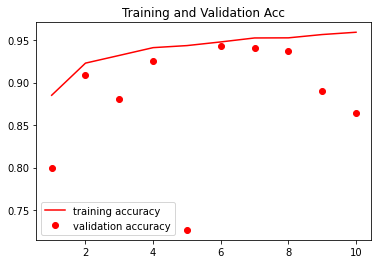
\includegraphics[width=1\textwidth,height=5cm,keepaspectratio]{Images/RadiographyCNNResNet50V2TrainAndValAccAugmentedDCGAN.png}\\
    \caption{Radiography Augmented ResNet50V2 Model DCGAN Accuracy - The X-Axis shows the epoch number and the Y-axis shows the accuracy}
    \label{fig:Radiography Augmented ResNet50V2 Model DCGAN Accuracy}
\end{figure}
 \begin{figure}[H]
    \centering
    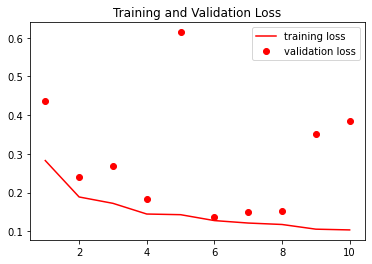
\includegraphics[width=1\textwidth,height=5cm,keepaspectratio]{Images/RadiographyCNNResNet50V2TrainAndValLossAugmentedDCGAN.png}\\
    \caption{Radiography Augmented ResNet50V2 Model DCGAN Loss - The X-Axis shows the epoch number and the Y-axis shows the loss}
    \label{fig:Radiography Augmented ResNet50V2 Model DCGAN Loss}
\end{figure}
\subsubsection{Radiography EfficentNetV2S Model}
The augmented EfficentNetV2S Model completed training with a final training set accuracy of 0.9640, with a training set loss of 0.0910 alongside a validation set accuracy of 0.9553 and a validation loss of 0.1167.  The model also had a test set accuracy of 0.9604 and a test set loss of 0.1056.  In contrast the original model attained a final training set accuracy 0.9383  of and a training set loss of 0.1519 alongside a validation accuracy of 0.8844 and a validation loss of 0.3362.  The original model also achieved a test set accuracy of 0.8811 and a test set loss of 0.3217.  This shows that the augmented model's training set accuracy increased by 0.0257 and its training set loss decreased by 0.0609 and the validation set accuracy increased by 0.0709 and its validation loss decreased by 0.2195.  The test set also improved in terms of loss and accuracy with an accuracy increase of 0.0794 and a loss decrease of 0.2161.   The augmented model has shown clear improvements when compared with the base model however, as shown from the images below early stopping could have helped improve the accuracy for the validation set. Figure \ref{fig:Radiography Augmented EfficientNetV2S Model DCGAN Accuracy} shows the training and validation accuracy and figure \ref{fig:Radiography Augmented EfficientNetV2S Model DCGAN Loss} shows the training and validation loss.
 \begin{figure}[H]
    \centering    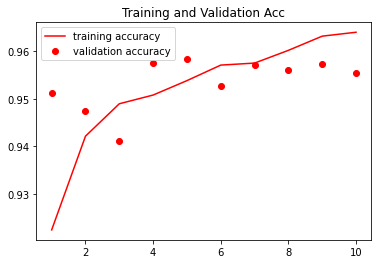
\includegraphics[width=1\textwidth,height=5cm,keepaspectratio]{Images/EfficientNetV2SBaselineTrainingValidationAccRadiographyAugmentedDCGAN.png}\\
    \caption{Radiography Augmented EfficientNetV2S Model DCGAN Accuracy The X-Axis shows the epoch number and the Y-axis shows the accuracy} 
    \label{fig:Radiography Augmented EfficientNetV2S Model DCGAN Accuracy}
\end{figure}
 \begin{figure}[H]
    \centering
    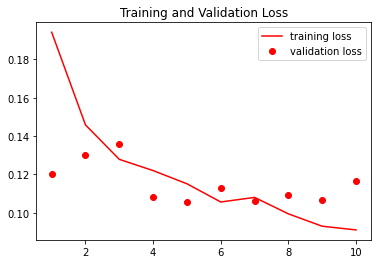
\includegraphics[width=1\textwidth,height=5cm,keepaspectratio]{Images/EfficientNetV2SBaselineTrainingValidationLossRadiographyAugmentedDCGAN.png}\\
    \caption{Radiography Augmented EfficientNetV2S Model DCGAN Loss - The X-Axis shows the epoch number and the Y-axis shows the loss}
    \label{fig:Radiography Augmented EfficientNetV2S Model DCGAN Loss}
\end{figure}
\subsubsection{Evaluation of Radiography Models}
Most of the radiography models showed a clear improvement across all sets when training on the augmented datasets.  The models which performed worse only suffered from a slight decrease in performance in terms of accuracy but had a decrease in loss which means the model may not have predicted all the cases correctly but was more confident in doing so.  The increase in confidence of all the radiography models could avoid situations where patients are unnecessarily quarantined.  The results from this dataset are significant in that they show a clear improvement across all models.
\subsection{Extensive CNN Models}
The Extensive CT dataset was augmented by 2,700 images and the augmented dataset has a total of 10,754 images, the original Extensive CT dataset had 8,054 images.  The original Extensive X-ray dataset had a total of 9,537 images which was increased to 10,537 when augmented, in total an additional 1,180 images were added to the augmented dataset.
\subsubsection{Extensive CNN CT Baseline Model}
The Extensive CNN CT baseline model attained a final training set accuracy of 0.9199 and a final training set loss of 0.1839 along with a final validation set accuracy of 0.5333 and a validation set loss of 3.4314  when the dataset was augmented.  The model  also had a test set loss of 3.2788  and a test set accuracy of  0.5373. In comparison to the original model which had a training set accuracy of 0.9023 and a training set loss of 0.2286 and a validation set accuracy of 0.8150 and a validation set loss of 0.3837  when trained for the same amount of epochs on a non-augmented set.  The original model also had a test set accuracy of 0.8319 and a test set loss of 0.3574.  Overall the augmented model performed better on the training set but worse on both the validation and test sets.  The training set accuracy increased by 0.0176 and the training set loss decreased by 0.0447 along with the validation set accuracy decreasing by 0.2817 and the loss increasing by 3.0477. The test set accuracy also declined by 0.2946 and the loss increased by 2.9206.  The training and validation set accuracy along with the training and validation set loss of this model are shown below.  The model appears to have a significant decrease in accuracy on the 10th epoch early stopping may have improved the overall accuracy.  Figure \ref{fig:Extensive CT Augmented Baseline Model DCGAN Accuracy} shows the training and validation accuracy and figure \ref{fig:Extensive CT Augmented Baseline Model DCGAN Loss} shows the training and validation loss.
 \begin{figure}[H]
    \centering    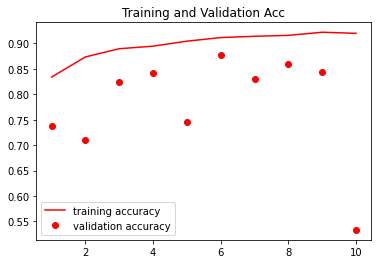
\includegraphics[width=1\textwidth,height=5cm,keepaspectratio]{Images/ExtensiveCNNBaselineModelExtensiveCovidAccCTAugmentedDCGAN.png}\\
    \caption{Extensive CT Augmented Baseline Model DCGAN Accuracy - The X-Axis shows the epoch number and the Y-axis shows the accuracy}
    \label{fig:Extensive CT Augmented Baseline Model DCGAN Accuracy}
\end{figure}
 \begin{figure}[H]
    \centering
    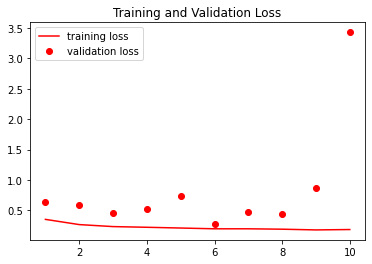
\includegraphics[width=1\textwidth,height=5cm,keepaspectratio]{Images/ExtensiveCNNBaselineModelExtensiveCovidLossCTAugmentedDCGAN.png}\\
    \caption{Extensive CT Augmented Baseline Model DCGAN - The X-Axis shows the epoch number and the Y-axis shows the loss}
    \label{fig:Extensive CT Augmented Baseline Model DCGAN Loss}
\end{figure}
\subsubsection{Extensive CNN CT Xception Model}
The Extensive CNN CT Xception model attained a final training set accuracy of 0.9920 and a final training set loss of 0.0278 along with a final validation set accuracy of 0.9704 and a validation set loss of 0.0777 when the dataset was augmented.  The model also has a test set accuracy of 0.9688 and a test set loss of 0.1054.  In comparison to the original model which had a training set accuracy of 0.9904  and a training set loss of 0.0238 and a validation set accuracy of 0.9534 and a validation set loss of 0.2250 when trained for the same amount of epochs on a non-augmented set.  The original model also had a test set accuracy of 0.9538 and a test set loss of 0.1772.  The augmented model performed better on all sets.  The training set accuracy increased by 0.0016 and the training set loss decreased by 0.1494. The validation set accuracy increased by 0.017 and the loss decreased by 0.1472. The test set accuracy also increased by 0.015 and the test set loss decreased by 0.0717.  Early stopping would have improved accuracy on the validation set as shown in the figures below which may in turn have improved the test set accuracy.  Figure \ref{fig:Extensive CT Augmented Xception Model DCGAN Accuracy} shows the training and validation accuracy and figure \ref{fig:Extensive CT Augmented Xception Model DCGAN Loss} shows the training and validation loss.
 \begin{figure}[H]
    \centering    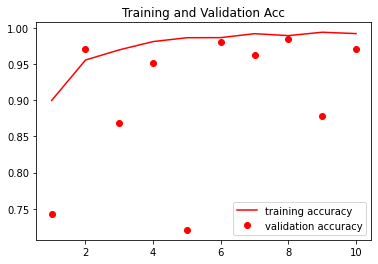
\includegraphics[width=1\textwidth,height=5cm,keepaspectratio]{Images/XceptionBaselineTrainingValidationAccuracyExtensiveCTAugmentedDCGAN.png}\\
    \caption{Extensive CT Augmented Xception Model DCGAN Accuracy - The X-Axis shows the epoch number and the Y-axis shows the accuracy}
    \label{fig:Extensive CT Augmented Xception Model DCGAN Accuracy}
\end{figure}
 \begin{figure}[H]
    \centering
    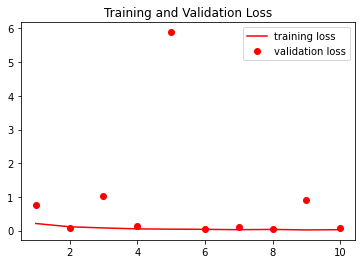
\includegraphics[width=1\textwidth,height=5cm,keepaspectratio]{Images/XceptionBaselineTrainingValidationLossExtensiveCTAugmentedDCGAN.png}\\
    \caption{Extensive CT Augmented Xception Model DCGAN Loss - The X-Axis shows the epoch number and the Y-axis shows the loss}
    \label{fig:Extensive CT Augmented Xception Model DCGAN Loss}
\end{figure}
\subsubsection{Extensive CNN CT ResNet50V2 Model}
The Extensive CNN CT ResNet50V2 model attained a final training set accuracy of 0.9485 and a final training set loss of 0.1255 along with a final validation set accuracy of 0.6091 and a validation set loss of 1.1563 when the dataset was augmented.  The model also has a test set accuracy of 0.6040 and a test set loss of 1.1806.  In comparison to the original model which had a training set accuracy of 0.9604 and a training set loss of 0.1140 and a validation set accuracy of 0.9350 and a validation set loss of 0.2078  when trained for the same amount of epochs on a non-augmented set.  The original model also had a test set accuracy of 0.9262 and a test set loss of 0.1993.  The augmented model performed worse on all sets.  The training set accuracy decreased by 0.0119 and the training set loss increased by 0.0115. The validation set accuracy decreased by 0.3259 and the validation set loss increased by 0.9485. The test accuracy also decreased by 0.3222 and the test loss increased by 0.9807.  Early stopping may have improved accuracy on the training and validation sets as shown in the figures below which may in turn have improved the test set accuracy.  Figure \ref{fig:Extensive CT Augmented ResNet50V2 Model DCGAN Accuracy} shows the training and validation accuracy and figure \ref{fig:Extensive CT Augmented ResNet50V2 Model DCGAN Loss} shows the training and validation loss.
 \begin{figure}[H]
    \centering    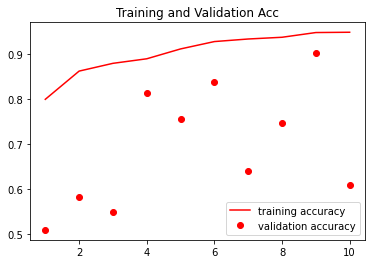
\includegraphics[width=1\textwidth,height=5cm,keepaspectratio]{Images/ResNet50V2BaselineTrainingValidationAccuracyExtensiveCTAugmentedDCGAN.png}\\
    \caption{Extensive CT Augmented ResNet50V2 Model DCGAN Accuracy - The X-Axis shows the epoch number and the Y-axis shows the accuracy}
    \label{fig:Extensive CT Augmented ResNet50V2 Model DCGAN Accuracy}
\end{figure}
 \begin{figure}[H]
    \centering
    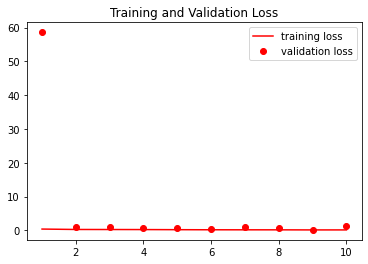
\includegraphics[width=1\textwidth,height=5cm,keepaspectratio]{Images/ResNet50V2BaselineTrainingValidationLossExtensiveCTAugmentedDCGAN.png}\\
    \caption{Extensive CT Augmented ResNet50V2 Model DCGAN Loss - The X-Axis shows the epoch number and the Y-axis shows the loss}
    \label{fig:Extensive CT Augmented ResNet50V2 Model DCGAN Loss}
\end{figure}
\subsubsection{Extensive CNN CT EfficientNetV2S Model}
The Extensive CNN CT EfficientNetV2S model attained a final training set accuracy of 0.9957 and a final training set loss of 0.0150 along with a final validation accuracy of 0.9815 and a validation set loss of 0.0634  when the dataset was augmented.  The augmented model also has a test accuracy of 0.9790 and a test loss of 0.0874.  In comparison to the original model which had a training set accuracy of 0.9901 and a training set loss of 0.0291 and a validation set accuracy of 0.9375 and a validation set loss of 0.2638 when trained for the same amount of epochs on a non-augmented set.  The original model also has a test set accuracy of 0.9437 and a test set loss of 0.2353.  The model performed better on all sets when training on the augmented set.  The training accuracy increased by 0.0056 and the training loss decreased by 0.0141. The validation accuracy increased by 0.044 and the loss decreased by 0.2004.  The test set accuracy increased by 0.0352 and the test set loss decreased by 0.1479.  This is an improvement over the original model on all sets which is a significant result.  Figure \ref{fig:Extensive CT Augmented EfficientNetV2S Model DCGAN Accuracy} shows the training and validation accuracy and figure \ref{fig:Extensive CT Augmented EfficientNetV2S Model DCGAN Loss} shows the training and validation loss.

 \begin{figure}[H]
    \centering    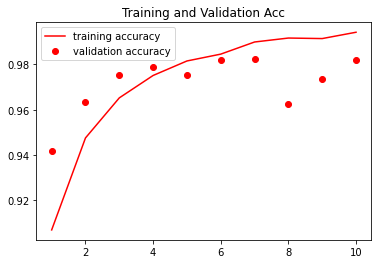
\includegraphics[width=1\textwidth,height=5cm,keepaspectratio]{Images/EfficientNetV2STrainingValidationAccuracyExtensiveCTAugmentedDCGAN.png}\\
    \caption{Extensive CT Augmented EfficientNetV2S Model DCGAN Accuracy - The X-Axis shows the epoch number and the Y-axis shows the accuracy}
    \label{fig:Extensive CT Augmented EfficientNetV2S Model DCGAN Accuracy}
\end{figure}
 \begin{figure}[H]
    \centering
    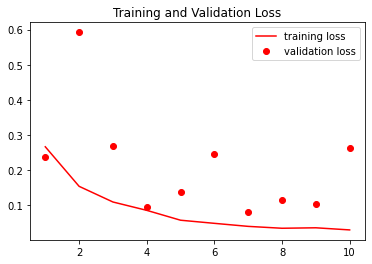
\includegraphics[width=1\textwidth,height=5cm,keepaspectratio]{Images/EfficientNetV2SBaselineTrainingValidationLossExtensiveCT.png}\\
    \caption{Extensive CT Augmented EfficientNetV2S Model DCGAN - The X-Axis shows the epoch number and the Y-axis shows the loss}
    \label{fig:Extensive CT Augmented EfficientNetV2S Model DCGAN Loss}
\end{figure}
\subsubsection{Evaluation of Extensive CNN CT Models}
The extensive CT models had mixed results when training on the augmented set.  The baseline model performed worse as did the ResNet50V2 model although the Xception and EfficientNetV2S models showed improvements across all sets.  Early stopping may have improved the accuracy for the Baseline and ResNet50V2 models as shown in the figures showing the validation and training accuracy and losses, it appears that the models may have been overtrained when training for the same number of epochs as the original given there is more data in the augmented sets.  The baseline model shows clear signs of overtraining as there is a large loss in accuracy and a large increase in loss on the 10th epoch and the ResNet50V2 model shows a large drop in accuracy on the 10th epoch as well.
\subsubsection{Extensive CNN X-ray Baseline Model}
The Extensive CNN X-ray baseline model attained a final training set accuracy of 0.9257 and a final training set loss of 0.1911 along with a final validation set accuracy of 0.7741 and a validation set loss of 1.1363 when the dataset was augmented. The augmented model also had a test set accuracy of 0.7784 and a test set loss of 1.0640.  In comparison to the original model which had a training set accuracy of 0.9278 and a training set loss of 0.1948 in addition to a validation set accuracy of 0.8587 and a validation set loss of 0.3482  when trained for the same amount of epochs on a non-augmented set.  The original model also had a test set accuracy of 0.8698 and a test set loss of 0.3203.  The model performed worse on all sets when trained on the augmented set.  The training set accuracy decreased by 0.0021 and the training set loss decreased by 0.0037. The validation set accuracy decrease by 0.0846 and the validation set loss increased by 0.7881.  The test set accuracy decreased by 0.0914 and the test set loss increased by 0.7437.
 \begin{figure}[H]
    \centering    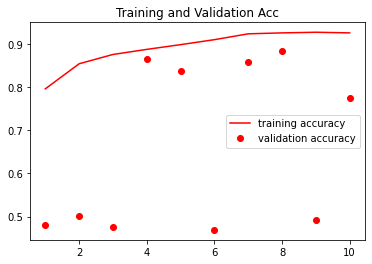
\includegraphics[width=1\textwidth,height=5cm,keepaspectratio]{Images/BaselineTrainingValidationAccuracyExtensiveXRayAugmentedDCGAN.png}\\
    \caption{Extensive X-ray Augmented Baseline Model DCGAN Accuracy - The X-Axis shows the epoch number and the Y-axis shows the accuracy}
    \label{fig:Extensive X-ray Augmented Baseline Model DCGAN Accuracy}
\end{figure}
 \begin{figure}[H]
    \centering
    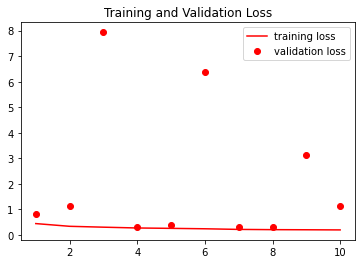
\includegraphics[width=1\textwidth,height=5cm,keepaspectratio]{Images/BaselineTrainingValidationLossExtensiveXRayAugmentedDCGAN.png}\\
    \caption{Extensive X-ray Augmented Baseline Model DCGAN Loss - The X-Axis shows the epoch number and the Y-axis shows the loss}
    \label{fig:Extensive X-ray Baseline Model DCGAN Loss}
\end{figure}
\subsubsection{Extensive CNN X-ray Xception Model}
The Extensive CNN X-ray Xception model attained a final training set accuracy of 0.9864 and a final training set loss of 0.0304 along with a final validation set accuracy of 0.9581 and a validation set loss of 0.2502 when the dataset was augmented.  The augmented model also has a test set accuracy of 0.9659 and a test set loss of 0.2254.  In comparison to the original model which had a training set accuracy of 0.9876 and a training set loss of 0.0277 in addition to a validation set accuracy of 0.9416 and a validation set loss of 0.2814 when trained for the same amount of epochs on a non-augmented set.  The original model also has a test set accuracy of 0.9578 and a test set loss of 0.1948.  The model performed slightly worse on the training set but better on both the validation set and on the test set when training on the augmented set.  The training set accuracy decreased by 0.0012 and the training set loss increased by 0.0027. The validation set accuracy increased by 0.0165 and the validation set loss decreased by 0.0312.  The test set accuracy increased by 0.0081 and the test set loss increased by 0.0306. The augmented and original model are fairly close in terms of accuracy and loss with the augmented model performing worse on the training set by a small margin but the model performed better on the validation and test sets in terms of accuracy by a small margin although the loss for the test set is slightly higher in the augmented model. Figure \ref{fig:Extensive X-ray Augmented Xception Model DCGAN Accuracy} shows the training and validation accuracy and figure \ref{fig:Extensive X-ray Augmented Xception Model DCGAN Loss} shows the training and validation loss.
 \begin{figure}[H]
    \centering    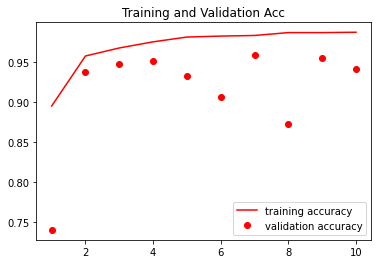
\includegraphics[width=1\textwidth,height=5cm,keepaspectratio]{Images/XceptionBaselineTrainingValidationAccuracyExtensiveXray.png}\\
    \caption{Extensive X-ray Augmented Xception Model DCGAN Accuracy - The X-Axis shows the epoch number and the Y-axis shows the accuracy}
    \label{fig:Extensive X-ray Augmented Xception Model DCGAN Accuracy}
\end{figure}
 \begin{figure}[H]
    \centering
    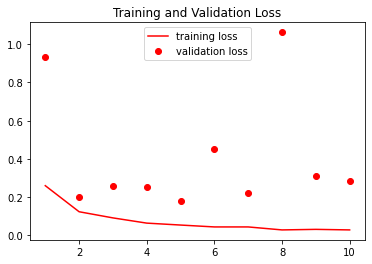
\includegraphics[width=1\textwidth,height=5cm,keepaspectratio]{Images/XceptionBaselineTrainingValidationLossExtensiveXray.png}\\
    \caption{Extensive X-ray Augmented Xception Model DCGAN Loss - The X-Axis shows the epoch number and the Y-axis shows the loss}
    \label{fig:Extensive X-ray Augmented Xception Model DCGAN Loss}
\end{figure}
\subsubsection{Extensive CNN X-ray ResNet50V2 Model}
The Extensive CNN X-ray ResNet50V2 model attained a final training set accuracy of 0.9687 and a final training set loss of 0.0852 along with a final validation set accuracy of 0.8275 and a validation set loss of 0.4574 when the dataset was augmented.  The augmented model also achieved an accuracy of 0.8210 for the test set along with a test set loss of 0.4680.  In comparison to the original model which has a training set accuracy of 0.9649 and a training set loss of 0.0907 in addition to a validation set accuracy of 0.9139 and a validation set loss of 0.9139 when trained for the same amount of epochs on a non-augmented set.  The original model also had a test set accuracy of 0.9224 and a test set loss of 0.2379.  The model performed worse on all sets when training on the augmented set.  The training set accuracy decreased by 0.0038 and the training set loss decreased by 0.0055. The validation set accuracy decreased by 0.0864 and the validation set loss increased by 0.1732.  Test set accuracy decreased by 0.1014 and the test set loss increased by 0.2301.
 \begin{figure}[H]
    \centering    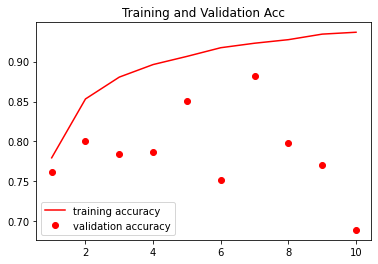
\includegraphics[width=1\textwidth,height=5cm,keepaspectratio]{Images/ResNet50V2BaselineTrainingValidationAccuracyExtensiveXray.png}\\
    \caption{Extensive X-ray Augmented ResNet50V2 Model DCGAN Accuracy - The X-Axis shows the epoch number and the Y-axis shows the accuracy}
    \label{fig:Extensive X-ray Augmented ResNet50V2 Model DCGAN Accuracy}
\end{figure}
 \begin{figure}[H]
    \centering
    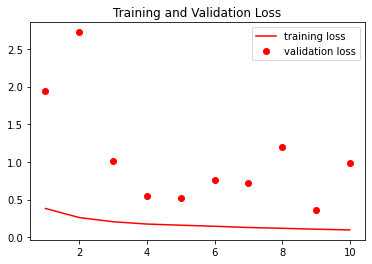
\includegraphics[width=1\textwidth,height=5cm,keepaspectratio]{Images/ResNet50V2BaselineTrainingValidationLossExtensiveXrayAugmentedDCGAN.png}\\
    \caption{Extensive X-ray Augmented ResNet50V2 Model DCGAN Loss - The X-Axis shows the epoch number and the Y-axis shows the loss}
    \label{fig:Extensive X-ray Augmented ResNet50V2 Model DCGAN Loss}
\end{figure}
\subsubsection{Extensive CNN X-ray EfficientNetV2S Model}
The Extensive CNN X-ray EfficientNetV2S model attained a final training set accuracy of 0.9864 and a final training set loss of 0.0366 along with a final validation set accuracy of 0.9695 and a validation set loss of 0.1686 when the dataset was augmented.  The model also has a test set accuracy of 0.9697 and a test set loss of 0.1579.  In comparison to the original model which had a training set accuracy of 0.9840 and a training set loss of 0.0396 in addition to a validation set accuracy of 0.9702 and a validation set loss of 0.1603 when trained for the same amount of epochs on a non-augmented set.  The original model also has a test set accuracy of 0.9766 and a test set loss of 0.1513.  The model performed slightly worse on all sets except the training set when training on the augmented set.  The training set accuracy increased by 0.0024 and the training set loss decreased by 0.003. The validation set accuracy decreased by 0.0007 and the validation set loss increased by 0.0083.  The test set accuracy decreased by 0.0069 and the test set loss increased by 0.0066.  It appears from analyzing these models that the quality of the X-ray images don't match the quality of the CT images as all the X-ray models performed worse than the originals. Figure \ref{fig:Extensive X-ray Augmented EfficientNetV2S Model DCGAN Accuracy} shows the training and validation accuracy and figure \ref{fig:Extensive X-ray Augmented EfficientNetV2S Model DCGAN Loss} shows the training and validation loss.
 \begin{figure}[H]
    \centering    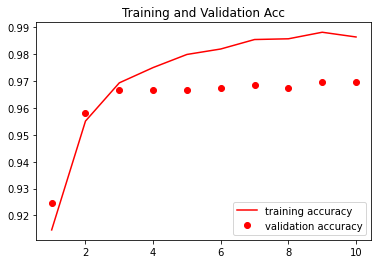
\includegraphics[width=1\textwidth,height=5cm,keepaspectratio]{Images/EfficientNetV2SBaselineTrainingValidationAccuracyExtensiveXRayAugmentedDCGAN.png}\\
    \caption{Extensive X-ray Augmented EfficientNetV2S Model DCGAN Accuracy - The X-Axis shows the epoch number and the Y-axis shows the accuracy}
    \label{fig:Extensive X-ray Augmented EfficientNetV2S Model DCGAN Accuracy}
\end{figure}
 \begin{figure}[H]
    \centering
    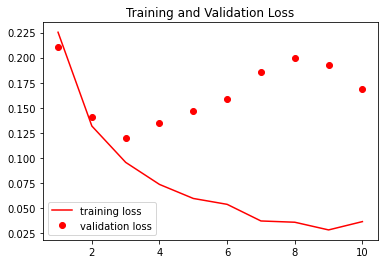
\includegraphics[width=1\textwidth,height=5cm,keepaspectratio]{Images/EfficientNetV2SBaselineTrainingValidationLossExtensiveXRayAugmentedDCGAN.png}\\
    \caption{Extensive X-ray Augmented EfficientNetV2S Model DCGAN Loss - The X-Axis shows the epoch number and the Y-axis shows the loss}
    \label{fig:Extensive X-ray Augmented EfficientNetV2S Model DCGAN Loss}
\end{figure}
\subsubsection{Evaluation of Extensive CNN X-ray Models}
Most of the Extensive X-ray CNN models performed worse in terms of accuracy and loss bar the Xception model which had slight improvements to both accuracy and loss.  The reason for the poor performance may be due to the variety in the X-ray images for this dataset as some X-rays are taken from the side and others are taken when the patient is facing forward. The poor performance could also have been caused by the quality of the augmented data.  When analyzing the output of the GAN for the X-ray model it appears that a lot of the images are grainy and lacking in quality.  The CT models on the other hand showed a clear improvement as the data generated from that set may suffer from grain and artifacts but the synthetic images share a lot of features with the original images.
\subsection{X-ray COVID-19 dataset CNN Models}
This dataset was augmented with 2000 artificially generated images, 1000 belonging to the pneumonia class and the other 1000 belonging to the normal class.  The augmented images were used only in training the models. Given the limited size of the dataset if we were to include augmented images in the validation set it would greatly skew the results as we would be gauging the model's ability to predict synthetic images as opposed to real images.  The limited size of the validation set for these models means that their performance is open to scrutiny.  The transfer learning models for this model include an additional layer of 1024 units with a ReLU activation function and another layer of 1 unit with a Sigmoid activation function.  The total size of the augmented set amounts to 2,148 images, the original dataset contained only 188 images. 
\subsubsection{X-ray COVID-19 Baseline Model}
The X-ray COVID-19 Baseline model attained a final training set accuracy of 0.9926 and a final training set loss of 0.0207 along with a final validation set accuracy of 0.5000 and a validation set loss of 5.2546 when the dataset was augmented.  The model also has a test set accuracy of 0.4375 and a test set loss of 6.2093.  In comparison to the original model which had a training set accuracy of 0.9122 and a training set loss of 0.2651 in addition to a validation set accuracy of 0.5000 and a validation set loss of 0.7918 when trained for the same amount of epochs on a non-augmented set.  The model performed worse on the validation and test sets in terms of accuracy when training on the augmented set but the augmented model had a higher accuracy and lower loss for the training set.  The training set accuracy increased by 0.0804 and the training set loss decreased by 0.2444. The validation set accuracy stayed the same at 0.5000 and the validation set loss increased by 4.4628.  The test set accuracy decreased by 0.0313 and the test set loss increased by 5.392.  Early stopping may have helped this model as the loss is a lot lower at epoch 8 and 9 for the validation set and has a higher validation accuracy with similar training accuracy.  Figure \ref{fig:X-ray COVID-19 Augmented Baseline Model DCGAN Accuracy} shows the training and validation accuracy and figure \ref{fig:X-ray COVID-19 Augmented Baseline Model DCGAN Loss} shows the training and validation loss.
 \begin{figure}[H]
    \centering    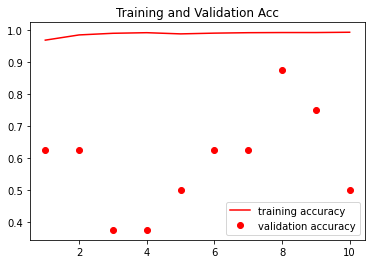
\includegraphics[width=1\textwidth,height=5cm,keepaspectratio]{Images/X-ray COVID-19 dataset CNN Train and Val Acc Augmented DCGAN.png}\\
    \caption{X-ray COVID-19 Augmented Baseline Model DCGAN Accuracy - The X-Axis shows the epoch number and the Y-axis shows the accuracy}
    \label{fig:X-ray COVID-19 Augmented Baseline Model DCGAN Accuracy}
\end{figure}
 \begin{figure}[H]
    \centering
    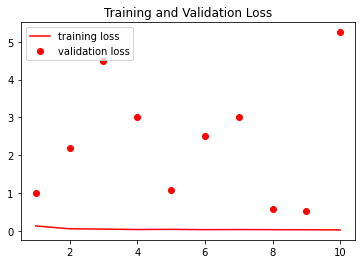
\includegraphics[width=1\textwidth,height=5cm,keepaspectratio]{Images/X-ray COVID-19 dataset CNN Train and Val Loss Augmented DCGAN.png}\\
    \caption{X-ray COVID-19 Augmented Baseline Model DCGAN Loss - The X-Axis shows the epoch number and the Y-axis shows the loss}
    \label{fig:X-ray COVID-19 Augmented Baseline Model DCGAN Loss}
\end{figure}
%Need to update stats in these models
\subsubsection{X-ray COVID-19 Xception Model}
The X-ray COVID-19 Xception model attained a final training set accuracy of 1.0000 and a final training set loss of 0.000047 along with a final validation set accuracy of 0.8750 and a validation set loss of 0.1786 when the dataset was augmented.  The model also achieved a test set accuracy of 0.8438 and a test set loss of 0.5912.  In comparison to the original model which had a training set accuracy of 0.9662 and a training set loss of 0.0951 in addition to a validation set accuracy of 0.5000 and a validation set loss of 5.4697 when trained for the same amount of epochs on a non-augmented set.  The original model also has a test set accuracy of 0.3750 and a test set loss of 7.5530 .  The model performed better on all sets in terms of accuracy when training on the augmented set.  The training set accuracy increased by 0.0338 and the training set loss decreased by 0.095053. The validation accuracy increased by 0.375 and the loss decreased by 5.2911.  The test set accuracy increased by 0.4688 and test set loss decreased by 6.9618.  Early stopping may help this model increase it's test set accuracy as the training loss is much lower at epochs 6 and 7 as is shown in the figures below.  Figure \ref{fig:X-ray COVID-19 Augmented Xception Model DCGAN Accuracy} shows the training and validation accuracy and figure \ref{fig:X-ray COVID-19 Augmented Xception Model DCGAN Loss} shows the training and validation loss.
 \begin{figure}[H]
    \centering    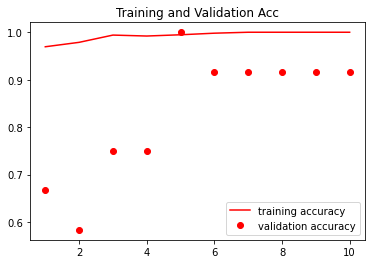
\includegraphics[width=1\textwidth,height=5cm,keepaspectratio]{Images/XceptionBaselineTrainingValidationAccuracyXRayCOVID19AugmentedDCGAN.png}\\
    \caption{X-ray COVID-19 Augmented Xception Model DCGAN Accuracy - The X-Axis shows the epoch number and the Y-axis shows the accuracy}
    \label{fig:X-ray COVID-19 Augmented Xception Model DCGAN Accuracy}
\end{figure}
 \begin{figure}[H]
    \centering
    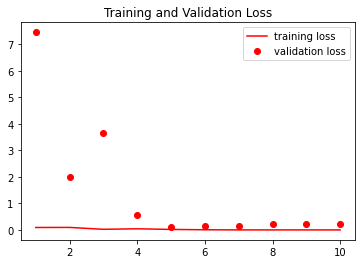
\includegraphics[width=1\textwidth,height=5cm,keepaspectratio]{Images/XceptionBaselineTrainingValidationLossXRayCOVID19AugmentedDCGAN.png}\\
    \caption{X-ray COVID-19 Augmented Baseline Model DCGAN Loss - The X-Axis shows the epoch number and the Y-axis shows the loss}
    \label{fig:X-ray COVID-19 Augmented Xception Model DCGAN Loss}
\end{figure}
\subsubsection{X-ray COVID-19 ResNet50V2 Model}
The X-ray COVID-19 ResNet50V2 model attained a final training set accuracy of 0.9846 and a final training set loss of 0.0565 along with a final validation set accuracy of 0.6250 and a validation loss of 1.4650 when the dataset was augmented.  The model also attained a test set accuracy of 0.6250 along with a test set loss of 2.0608.  In comparison to the original model which had a training set accuracy of 0.9257 and a training loss of 0.2622 in addition to a validation set accuracy of 0.3750 and a validation set loss of 29.2193 when trained for the same amount of epochs on a non-augmented set.  The original model also had a test set accuracy of 0.4688 and test set loss of 23.9440.  The model performed better on all sets in terms of both accuracy and loss.  The training set accuracy increased by 0.0589 and the training set loss decreased by 0.2057. The validation set accuracy increased by 0.25 and the validation set loss decreased by 27.7543.  The test set accuracy decreased by 0.15625 and the test set loss decreased by 21.88.  The model shows a significant improvement when compared to the non augmented model. As seen with previous models early stopping would have benefited this model as the training and validation accuracy is higher in earlier epochs.  Figure \ref{fig:X-ray COVID-19 Augmented ResNet50V2 Model DCGAN Accuracy} shows the training and validation accuracy and figure \ref{fig:X-ray COVID-19 Augmented ResNet50V2 Model DCGAN Loss} shows the training and validation loss.
 \begin{figure}[H]
    \centering    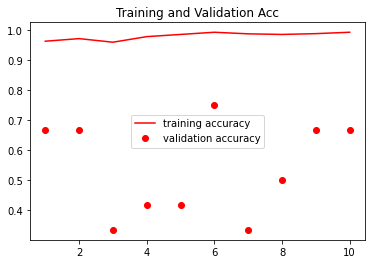
\includegraphics[width=1\textwidth,height=5cm,keepaspectratio]{Images/ResNet50V2BaselineTrainingValidationAccXRayCOVID19AugmentedDCGAN.png}\\
    \caption{X-ray COVID-19 Augmented ResNet50V2 Model DCGAN Accuracy - The X-Axis shows the epoch number and the Y-axis shows the accuracy}
    \label{fig:X-ray COVID-19 Augmented ResNet50V2 Model DCGAN Accuracy}
\end{figure}
 \begin{figure}[H]
    \centering
    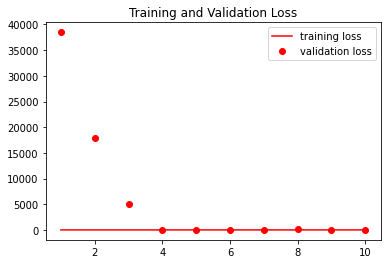
\includegraphics[width=1\textwidth,height=5cm,keepaspectratio]{Images/ResNet50V2BaselineTrainingValidationLossXRayCOVID19AugmentedDCGAN.png}\\
    \caption{X-ray COVID-19 Augmented ResNet50V2 Model DCGAN Loss - The X-Axis shows the epoch number and the Y-axis shows the loss}
    \label{fig:X-ray COVID-19 Augmented ResNet50V2 Model DCGAN Loss}
\end{figure}
\subsubsection{X-ray COVID-19 EfficientNetV2S Model}
The X-ray COVID-19 EfficientNetV2S model attained a final training set accuracy of 0.9981  and a final training set loss of 0.0091 along with a final validation set accuracy of 1.0000 and a validation set loss of 0.0106 when the dataset was augmented.  The model attained a test set accuracy of 0.9375 along with a test set loss of 0.1713.  In comparison to the original model which had a training set accuracy of 1.0000 and a training set loss of 0.0063 in addition to a validation set accuracy of 1.0000 and a validation set loss of 0.0011  when trained for the same amount of epochs on a non-augmented set.  The non augmented model also had a test set accuracy of 0.9375 and a test set loss of 0.2317.  The model performed better on the test set but slightly worse on the training set and validation set.  The training set accuracy decreased by 0.0019 and the training set loss increased by 0.0028. The validation set accuracy stayed the same and the validation set loss increased by 0.0095.  The test set accuracy stayed the same and the test set loss decreased by 0.0604.  Early stopping would have helped increase the training and validation scores as shown in the figures below.  Figure \ref{fig:X-ray COVID-19 Augmented EfficientNetV2S Model DCGAN Accuracy} shows the training and validation accuracy and figure \ref{fig:X-ray COVID-19 Augmented EfficientNetV2S Model DCGAN Loss} shows the training and validation loss.
 \begin{figure}[H]
    \centering    
    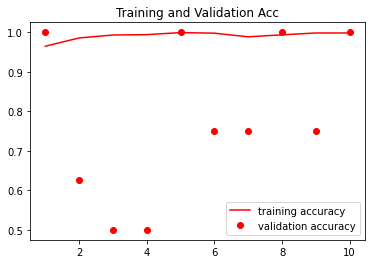
\includegraphics[width=1\textwidth,height=5cm,keepaspectratio]{Images/EfficientNetV2SBaselineTrainingValidationAccXRayCOVID19AugmentedDCGAN.png}\\
    \caption{X-ray COVID-19 Augmented EfficientNetV2S Model DCGAN Accuracy - The X-Axis shows the epoch number and the Y-axis shows the accuracy}
    \label{fig:X-ray COVID-19 Augmented EfficientNetV2S Model DCGAN Accuracy}
\end{figure}
 \begin{figure}[H]
    \centering
    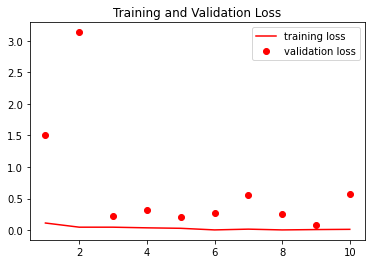
\includegraphics[width=1\textwidth,height=5cm,keepaspectratio]{Images/EfficientNetV2SBaselineTrainingValidationLossXRayCOVID19AugmentedDCGAN.png}\\
    \caption{X-ray COVID-19 Augmented EfficientNetV2S Model DCGAN Loss - The X-Axis shows the epoch number and the Y-axis shows the loss}
    \label{fig:X-ray COVID-19 Augmented EfficientNetV2S Model DCGAN Loss}
\end{figure}
\subsubsection{Evaluation of CNN models for X-ray COVID-19 Dataset}
Although some of the models do show improvement, the ability to evaluate the models is limited.  The original dataset is broken into images for train and test and the test set only contains 40 images.  It would be unwise to augment the test set as then we would have been comparing synthetic images with synthetic images, and given that the amount of images synthetically generated is far larger than the real data in the dataset, it would have greatly skewed the results.  Some of the models do show an improvement when compared with the original and those that perform worse than the original do so by a small margin.  The more data in the dataset the more features there are to detect so a small increase in loss and accuracy for these models is to be expected, especially given the small size of the dataset.  It was surprising to see that a few models here did outperform the original as the dataset used to train the GANs was limited to 188 images, although this could be due to the test data in the dataset also being used to train the GANs.  The model's performance may possibly have been improved by tweaking some of the hyper-parameters or adjusting the size of the added layer of 1024 units as the number of units added may have been too large.
\section{Evaluation of GAN Models}
In this section we will analyze the output for each GAN on the augmented classes of each dataset.  Some of the classes mentioned were not used to generate synthetic images for the models, as they were the majority class, but we thought they were worth discussing regardless.
\subsection{Radiography GAN Models}
\subsubsection{Radiography DCGAN for COVID-19 Class Augmentation}
The radiography DCGAN for synthetically generated COVID-19 samples had mixed results.  Some of the images generated by the DCGAN came out looking very similar to the masks of patients lungs which were in the database.  We have included a side by side comparison in figure \ref{fig:Real COVID-19 Radiography Mask Example} and \ref{fig:Synthetically Generated COVID-19 Radiography Mask(DCGAN)} below
 \begin{figure}[H]
    \centering
    \begin{subfigure}{.4\textwidth}
    \centering
      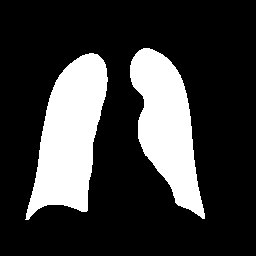
\includegraphics[width=.4\linewidth,keepaspectratio]{Images/Radiography_Real_Mask_COVID19_Example.png}
      \caption{Real COVID-19 Radiography Mask Example}
      \label{fig:Real COVID-19 Radiography Mask Example}
    \end{subfigure}\hfill%
    \begin{subfigure}{.4\textwidth}
    \centering
      
\includegraphics[width=.4\linewidth,keepaspectratio]{Images/Radiography_GAN_Mask_COVID19_Example.png}
      \caption{Generated COVID-19 Radiography Mask Example DCGAN}
      \label{fig:Synthetically Generated COVID-19 Radiography Mask(DCGAN)}
    \end{subfigure}\hfill%
\end{figure}
As shown in the above figures \ref{fig:Real COVID-19 Radiography Mask Example} and \ref{fig:Synthetically Generated COVID-19 Radiography Mask(DCGAN)}, the synthetically generated COVID-19 mask looks very similar to the example taken from the dataset.  However not every single generated image came out as well as those that we have shown for demonstration purposes.  From reviewing the generated images it appears that a number of images have some issues.  A common issue faced was images which were generated with artefacts and some images which were not up to standard with the images in the dataset.   
 \begin{figure}[H]
    \centering
    \begin{subfigure}{.4\textwidth}
    \centering
      
\includegraphics[width=.4\linewidth,keepaspectratio]{Images/ArtefactImageCOVID19MaskRadiographyDCGAN.png}
      \caption{Synthetically generated COVID 19 mask with Artefacts(DCGAN)}
      \label{fig:Image with Artefacts(Radiography DCGAN)}
    \end{subfigure}\hfill%
    \begin{subfigure}{.4\textwidth}
    \centering
      
\includegraphics[width=.4\linewidth,keepaspectratio]{Images/MalformedImageCOVID19MaskRadiographyDCGAN.png}
      \caption{Malformed Image of synthetically generated COVID 19 Mask(DCGAN)}
      \label{fig:Malformed Image of COVID 19 Mask(Radiography DCGAN)}
    \end{subfigure}\hfill%
\end{figure}
From training a number of models there appears to be a need for pruning out bad images generated by the GAN and determining which images resemble X-Rays and Masks and which are "garbage" images which don't resemble data in our dataset.  This will require a lot of manual effort in determining which generated images are worth including in the augmented dataset and which are worth throwing away.
\\
Similarly the augmentation of the X-ray images produced good results although, much like the synthetically generated masks, there were a number with artefacts and some images that were malformed.  We have included two images below to compare the synthetically generated example \ref{fig:Synthetically Generated COVID-19 Radiography X-ray(DCGAN)}  with a real example \ref{fig:Real COVID-19 Radiography X-ray Example} below
 \begin{figure}[H]
    \centering
    \begin{subfigure}{.35\textwidth}
    \centering
      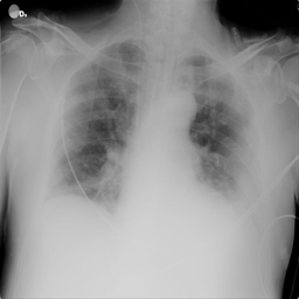
\includegraphics[width=.4\linewidth,keepaspectratio]{Images/ExampleofXrayRadiographyCOVID19.png}
      \caption{Real COVID-19 Radiography X-ray Example}
      \label{fig:Real COVID-19 Radiography X-ray Example}
    \end{subfigure}\hfill%
    \begin{subfigure}{.35\textwidth}
    \centering
      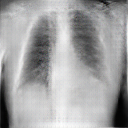
\includegraphics[width=.4\linewidth,keepaspectratio]{Images/SyntheticRadiographyXrayCOVID19Example.png}
      \caption{Generated COVID-19 Radiography X-ray Example DCGAN}
      \label{fig:Synthetically Generated COVID-19 Radiography X-ray(DCGAN)}
    \end{subfigure}\hfill%
\end{figure}
As shown in the above figures \ref{fig:Real COVID-19 Radiography X-ray Example} and \ref{fig:Synthetically Generated COVID-19 Radiography X-ray(DCGAN)} the two images look very similar to each other and there are clear similarities contained in the images.  Malformed images are also present in the generated data and two such examples have been shown in the figures below.
 \begin{figure}[H]
    \centering
    \begin{subfigure}{.35\textwidth}
    \centering
      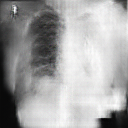
\includegraphics[width=.4\linewidth,keepaspectratio]{Images/MalformedCOVID19XrayImageExample1RadiographyDCGAN.png}
      \caption{Malformed COVID-19 Radiography X-ray Example Number 1 Radiography DCGAN}
      \label{fig:Malformed COVID-19 Radiography X-ray Example Number 1 Radiography DCGAN}
    \end{subfigure}\hfill%
    \begin{subfigure}{.35\textwidth}
    \centering
      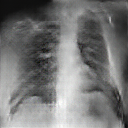
\includegraphics[width=.4\linewidth,keepaspectratio]{Images/MalformedCOVID19XrayImageExample2RadiographyDCGAN.png}
      \caption{Malformed COVID-19 Radiography X-ray Example Number 2 Radiography DCGAN}
      \label{fig:Malformed COVID-19 Radiography X-ray Example Number 2 Radiography DCGAN}
    \end{subfigure}\hfill%
\end{figure}
\subsubsection{Radiography DCGAN for Pneumonia Class Augmentation}
Much like in the previous section there was some success when augmenting the Pneumonia class despite it being a little less than half the size of the covid class (for reference the covid class contains 3,616 images in both the mask and X-ray folders where as the Pneumonia class contains 1,345 images in both the mask and X-ray folders).  Most of the masks generated resembled those in the dataset an example of a synthetically generated pneumonia mask\ref{fig:Synthetically Generated Pneumonia Radiography Mask(DCGAN)} alongside a real example mask\ref{fig:Real Pneumonia Radiography Mask Example} is visible in the figures below
 \begin{figure}[H]
    \centering
    \begin{subfigure}{.4\textwidth}
    \centering
      
\includegraphics[width=.4\linewidth,keepaspectratio]{Images/ExampleOfSyntheticallyGeneratedMaskPneumoniaCOVID19RadiographyDCGAN.png}
      \caption{Generated Pneumonia Radiography Mask Example DCGAN}
      \label{fig:Synthetically Generated Pneumonia Radiography Mask(DCGAN)}
    \end{subfigure}\hfill%
    \begin{subfigure}{.4\textwidth}
    \centering
      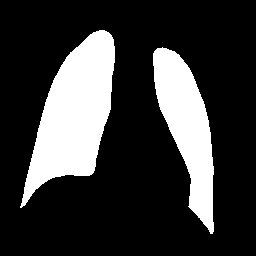
\includegraphics[width=.4\linewidth,keepaspectratio]{Images/ExampleOfPneumoniaMaskRadiographyCOVID19.png}
      \caption{Real Pneumonia Radiography Mask Example}
      \label{fig:Real Pneumonia Radiography Mask Example}
    \end{subfigure}\hfill%
\end{figure}
The X-ray DCGAN also produced convincing results which are shown below in figures \ref{fig:Real Pneumonia Radiography X-ray Example} which shows a real X-ray example from the dataset and \ref{fig:Synthetically Generated Pneumonia Radiography X-ray(DCGAN)}.
 \begin{figure}[H]
    \centering
    \begin{subfigure}{.4\textwidth}
    \centering
      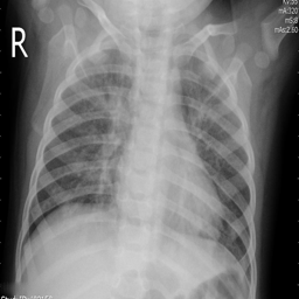
\includegraphics[width=.4\linewidth,keepaspectratio]{Images/ExampleOfPneumoniaXrayRadiographyCOVID19.png}
      \caption{Real Pneumonia Radiography X-ray Example}
      \label{fig:Real Pneumonia Radiography X-ray Example}
    \end{subfigure}\hfill%
    \begin{subfigure}{.4\textwidth}
    \centering
      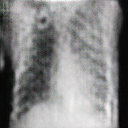
\includegraphics[width=.4\linewidth,keepaspectratio]{Images/ExampleOfSyntheticallyGeneratedXrayPneumoniaCOVID19RadiographyDCGAN.png}
      \caption{Generated Pneumonia Radiography X-ray Example DCGAN}
      \label{fig:Synthetically Generated Pneumonia Radiography X-ray(DCGAN)}
    \end{subfigure}\hfill%
\end{figure}
As shown in the above images \ref{fig:Real Pneumonia Radiography X-ray Example} and \ref{fig:Synthetically Generated Pneumonia Radiography X-ray(DCGAN)} there appears to be a number of similarities between the two images but the synthetically generated X-ray does appear to lack the quality of the original.
\\
In conclusion the malformed images may have a detrimental effect on the training and it would require a lot of manual effort and computational power to both prune the augmented dataset and retrain the GANs.  The examples above show that the DCGAN is a powerful method of generated synthetic data although it is not without its faults.
\subsection{Extensive X-Ray GAN Models}
The X-ray DCGAN models achieved some success when synthetically generating both the X-rays for COVID and X-rays of non-COVID patients.  The following images show a real example and a synthetic example side by side for comparison.
 \begin{figure}[H]
    \centering
    \begin{subfigure}{.4\textwidth}
    \centering
      \includegraphics[width=.4\linewidth,keepaspectratio]{Images/ExampleOfRealExtensiveCOVIDXray.png}
      \caption{Real COVID X-ray Example Extensive}
      \label{fig:Real COVID X-ray Example Extensive}
    \end{subfigure}\hfill%
    \begin{subfigure}{.4\textwidth}
    \centering
      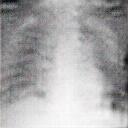
\includegraphics[width=.4\linewidth,keepaspectratio]{Images/ExampleOfSyntheticallyGeneratedCOVIDXrayExtensiveDCGAN.png}
      \caption{Synthetically Generated COVID X-ray Example Extensive DCGAN}
      \label{fig:Synthetically Generated COVID X-ray Example Extensive DCGAN}
    \end{subfigure}\hfill%
\end{figure}
As shown in the images above there are some similarities between the two X-rays although the synthetically generated example looks blurry and appears to be of low quality when compared with the real example.  Unlike the Radiography dataset where images appeared to share characteristics there seems to be a lot more variance in this dataset as some X-rays are taken from the side where as others are taken straight forward.  This is the reason that the synthetically generated images don't appear to match the quality of the synthetically generated radiography dataset images.
\\
When using the model to produce non-COVID X-rays there seemed to be slightly better results as is shown in the figures below \ref{fig:Real Non COVID X-ray Example Extensive} which is the real example from our dataset and in \ref{fig:Synthetically Generated Non COVID X-ray Example Extensive DCGAN} which is the synthetic example generated by the DCGAN.
 \begin{figure}[H]
    \centering
    \begin{subfigure}{.4\textwidth}
    \centering
      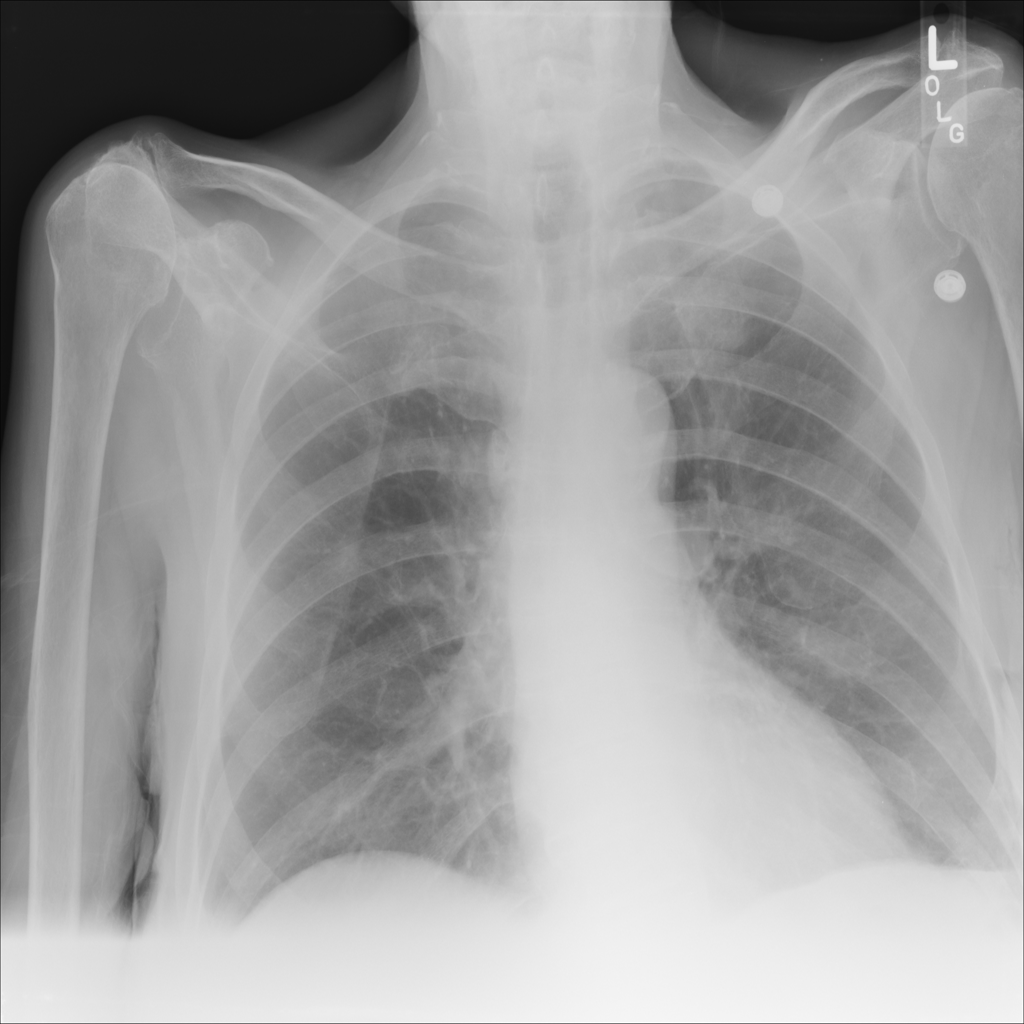
\includegraphics[width=.4\linewidth,keepaspectratio]{Images/ExampleOfNonCOVIDXray.png}
      \caption{Real Non COVID X-ray Example Extensive}
      \label{fig:Real Non COVID X-ray Example Extensive}
    \end{subfigure}\hfill%
    \begin{subfigure}{.4\textwidth}
    \centering
      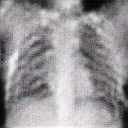
\includegraphics[width=.4\linewidth,keepaspectratio]{Images/ExampleOfSyntheticNonCOVIDXrayExtensiveDCGAN.png}
      \caption{Synthetically Generated Non COVID X-ray Example Extensive DCGAN}
      \label{fig:Synthetically Generated Non COVID X-ray Example Extensive DCGAN}
    \end{subfigure}\hfill%
\end{figure}
The reason for the synthetically generated non-COVID examples having more quality is that there seems to be less variance in X-ray images in the non-COVID class and also the non-COVID class is the majority in this dataset.
\\
There were also the issues of malformed images and artefacts when training these DCGANs like the previous examples shown in figures \ref{fig:Malformed Image of COVID 19 Mask(Radiography DCGAN)} and \ref{fig:Image with Artefacts(Radiography DCGAN)}
\subsection{Extensive CT GAN Models}
The CT GAN models had some issues reproducing the CT images this was due to their being a lot of variety in the CT dataset.  Included in the figures below is an example of a real COVID CT scan along with the synthetically generated COVID CT scan.
 \begin{figure}[H]
    \centering
    \begin{subfigure}{.4\textwidth}
    \centering
      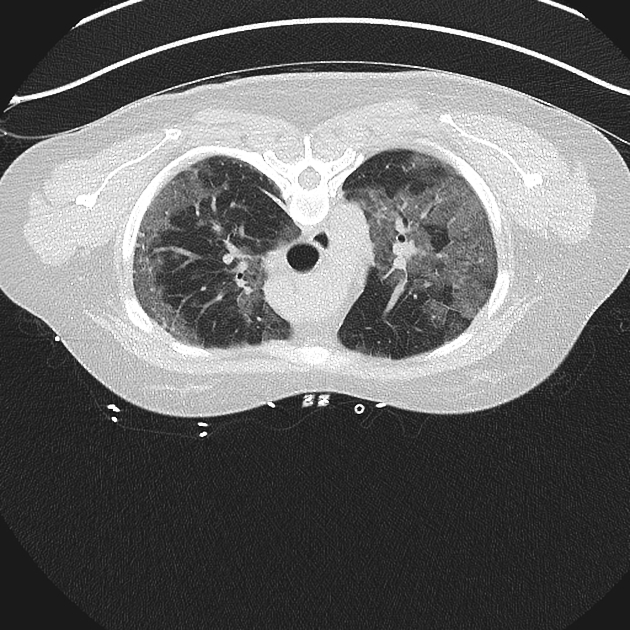
\includegraphics[width=.4\linewidth,keepaspectratio]{Images/COVIDCTScanExampleExtensive.png}
      \caption{Real COVID CT Example Extensive}
      \label{fig:Real COVID CT Example Extensive}
    \end{subfigure}\hfill%
    \begin{subfigure}{.4\textwidth}
    \centering
      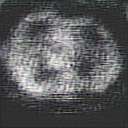
\includegraphics[width=.4\linewidth,keepaspectratio]{Images/ExampleOfSyntheticallyGeneratedCOVIDCTScanExtensiveDCGAN.png}
      \caption{Synthetically Generated COVID CT Example Extensive DCGAN}
      \label{fig:Synthetically Generated COVID CT Example Extensive DCGAN}
    \end{subfigure}\hfill%
\end{figure}
As shown in the figures above the synthetic example \ref{fig:Synthetically Generated COVID CT Example Extensive DCGAN} appears to be grainy and lacking in quality despite sharing some similar features with the real example \ref{fig:Real COVID CT Example Extensive}.  The poor quality may be caused by the variety of images in the dataset, as there are many differing features between the images in the dataset. 
\\
As with the COVID CT scans, the non-COVID CT scans had similar results which can be seen below
 \begin{figure}[H]
     \begin{subfigure}{.4\textwidth}
    \centering
      \includegraphics[width=.4\linewidth,keepaspectratio]{Images/ExampleOfSyntheticNonCOVIDCTScanExtensiveDCGAN.png}
      \caption{Synthetically Generated non COVID CT Example Extensive DCGAN}
      \label{fig:Synthetically Generated non COVID CT Example Extensive DCGAN}
    \end{subfigure}\hfill%
    \centering
    \begin{subfigure}{.4\textwidth}
    \centering
      \includegraphics[width=.4\linewidth,keepaspectratio]{Images/ExampleOfNonCOVIDCTScan.png}
      \caption{Real non COVID CT Example Extensive}
      \label{fig:Real non COVID CT Example Extensive}
    \end{subfigure}\hfill%
\end{figure}
The above figures show the lack of quality in the synthetically generated image\ref{fig:Synthetically Generated non COVID CT Example Extensive DCGAN} when compared with the example taken from the dataset \ref{fig:Real non COVID CT Example Extensive}. From trying a number of GAN architectures the same issue was seen with lack of quality augmented images being produced.  However the synthetic images do share some features with the real example.
\subsection{X-ray COVID-19 dataset GAN Models}
Surprisingly given the very small dataset the X-ray COVID-19 DCGANs produced relatively convincing images for both classes.  Below are two X-ray examples for the normal class one image is generated by the DCGAN and the other is taken from the dataset
 \begin{figure}[H]
    \centering
    \begin{subfigure}{.4\textwidth}
    \centering
      \includegraphics[width=.4\linewidth,keepaspectratio]{Images/ExampleOfNormalXrayXrayCOVID19Dataset.jpeg}
      \caption{Real Normal X-ray X-ray Dataset COVID-19}
      \label{fig:Real Normal X-ray X-ray Dataset COVID-19}
    \end{subfigure}\hfill%
    \begin{subfigure}{.4\textwidth}
    \centering
      \includegraphics[width=.4\linewidth,keepaspectratio]{Images/ExampleOfSyntheticallyGeneratedNormalXrayCOVID19XrayDatasetDCGAN.png}
      \caption{Synthetically Generated Normal X-ray X-ray Dataset COVID-19 DCGAN}
      \label{fig:Synthetically Generated Normal X-ray X-ray Dataset COVID-19 DCGAN}
    \end{subfigure}\hfill%
\end{figure}
As shown in the figures above the synthetically generated example \ref{fig:Synthetically Generated Normal X-ray X-ray Dataset COVID-19 DCGAN} lacks the quality of the original \ref{fig:Real Normal X-ray X-ray Dataset COVID-19} but appears to have similar features.  The next figures show an example of a synthetically generated pneumonia X-ray along with a sample taken from the dataset
 \begin{figure}[H]
    \centering
    \begin{subfigure}{.4\textwidth}
    \centering
      \includegraphics[width=.4\linewidth,keepaspectratio]{Images/ExampleOfPneumoniaXrayXrayCOVID19Dataset.jpeg}
      \caption{Real Pneumonia X-ray X-ray Dataset COVID-19}
      \label{fig:Real Pneumonia X-ray X-ray Dataset COVID-19}
    \end{subfigure}\hfill%
    \begin{subfigure}{.4\textwidth}
    \centering
      \includegraphics[width=.4\linewidth,keepaspectratio]{Images/ExampleOfSyntheticallyGeneratedPneumoniaXrayCOVID19XrayDatasetDCGAN.png}
      \caption{Synthetically Generated Pneumonia X-ray X-ray Dataset COVID-19 DCGAN}
      \label{fig:Synthetically Generated Pneumonia X-ray X-ray Dataset COVID-19 DCGAN}
    \end{subfigure}\hfill%
\end{figure}
The figure shown above \ref{fig:Synthetically Generated Pneumonia X-ray X-ray Dataset COVID-19 DCGAN} suffers from the same issue the synthetically generated images of the Normal class suffered from, in that the synthetic image appears grainy but does share some similar features with the original images \ref{fig:Real Pneumonia X-ray X-ray Dataset COVID-19}.  Given the limited size of the dataset used to train the GANs there was no need to experiment further as this seems to be the best quality a DCGAN can produce.
\subsection{Summary of Results}
In this section I will give a brief summary of the results from the research and their significance.  I will detail what has been achieved upon completion of the implementation of the AI models.
\subsubsection{Analysis of Results and Their Significance}
Overall a number of augmented models showed improvements in terms of both accuracy and loss.  This means that the augmented models performed better than the original models.  The increase in performance of the augmented models may provide advantages in this area and allow for doctors to more easily diagnose patients more accurately, which would in turn allow doctors to have more free-time to spend on other patients.  The results from this study could possibly be used in a number of fields and different areas other than the automated diagnosis of COVID-19 but more research will need to be done to gauge synthetically generated data in said areas and fields. 
\\
In comparison to the existing COVID automated diagnosis model viewed in the literature review which had accuracy of 99.4\%  none of the augmented or original models were able to surpass this performance.  The model which came closest was the augmented Extensive CNN CT EfficientNetV2S model which had a test set accuracy of 0.9697 or approximately 97\%.  When evaluating the performance it is important to remember that the size of the dataset plays a significant role, the literature review model was trained on a dataset with of 4,575 X-ray images, 1,525 of which were X-rays of COVID positive patients.  In comparison the Extensive COVID-19 CT dataset contains 2,628 Non-COVID CT scans and 5,427 COVID CT scans, the augmented dataset contained and additional 2,700 Non-COVID images which in total gives the dataset a size of 10,755 images which is an increase of 4,655 images.  Given that the model is exposed to more data it could be argued that this model would be more beneficial in a clinical setting given it is exposed to more features in the data which could be an improvement in terms of the model's ability to generalize.  The augmented radiography models also showed some decent performance compared to the model mentioned in the literature review with the top model getting a test set accuracy of 0.9604 or 96\% when trained on a far larger dataset of 60,933 images.   Some of the non-augmented models were also able to get close to the COVID-19 diagnostic model mentioned in the literature review while training on slightly larger datasets the Extensive COVID-19 X-ray model which had a test set accuracy of 0.9766 or approximately 98\% is a good example of this.
\\
The overall results of this study found that synthetic data was useful for some model architectures and improved a number of models but a number of models trained on the synthetic data performed poorly compared to models trained on real data.  It appears more research is needed in this area as computational limitations and lack of data pruning may have skewed the results negatively.  The variation of data also proved to be detrimental in some datasets which can be seen from the Extensive COVID-19 X-ray CNN models, the poor performance could be due to the variety of data present as some of the X-rays are taken from the side and others are taken from with the patient facing the camera.
\section{Conclusion}
In conclusion of this section we can see from the figures produced by the GANs that the models were able to reproduce convincing images which look close to their target domain.  We can also see that some images such as figures \ref{fig:Image with Artefacts(Radiography DCGAN)} and \ref{fig:Malformed Image of COVID 19 Mask(Radiography DCGAN)} have aberrations and artifacts which distort the image and could confuse the model when training on the synthetic data.  The only solution to this issue would be to prune each image manually which would take a lot of time and effort.  Due to time constraints we were unable to prune and curate each image.  The models could possibly be improved by removing malformed images or images with artifacts.  There is also the issue of image resolution which may have caused some models to perform worse than they normally would have if the images were standardized.  Due to computational limitations it was very difficult and time-consuming to train GANs to produce high resolution images.  Trying to produce images with high resolutions used a lot of computational power and often caused Colab to crash during training.  However, the augmented CNN models do show improvement on a number of datasets such as the Radiography and Extensive CT datasets.  Although the accuracy may be lower and the loss may be higher for some models the added data may be beneficial when applied in a clinical setting, as the augmented dataset adds more variety of images and more data to for the model to learn from to detect subtle features and characteristics.  It is important to remember the size of the datasets when gauging these models as it would be easier to achieve a much higher accuracy and lower loss on smaller datasets than it would on larger sets.  The overall results of this research do show that there is much improvement in terms of both loss and accuracy as is detailed in the previous section ``Analysis of Results and Their Significance``.